\documentclass[border=20pt, tikz]{standalone}
\usetikzlibrary{shapes.geometric, arrows.meta, positioning, calc, backgrounds}

\begin{document}
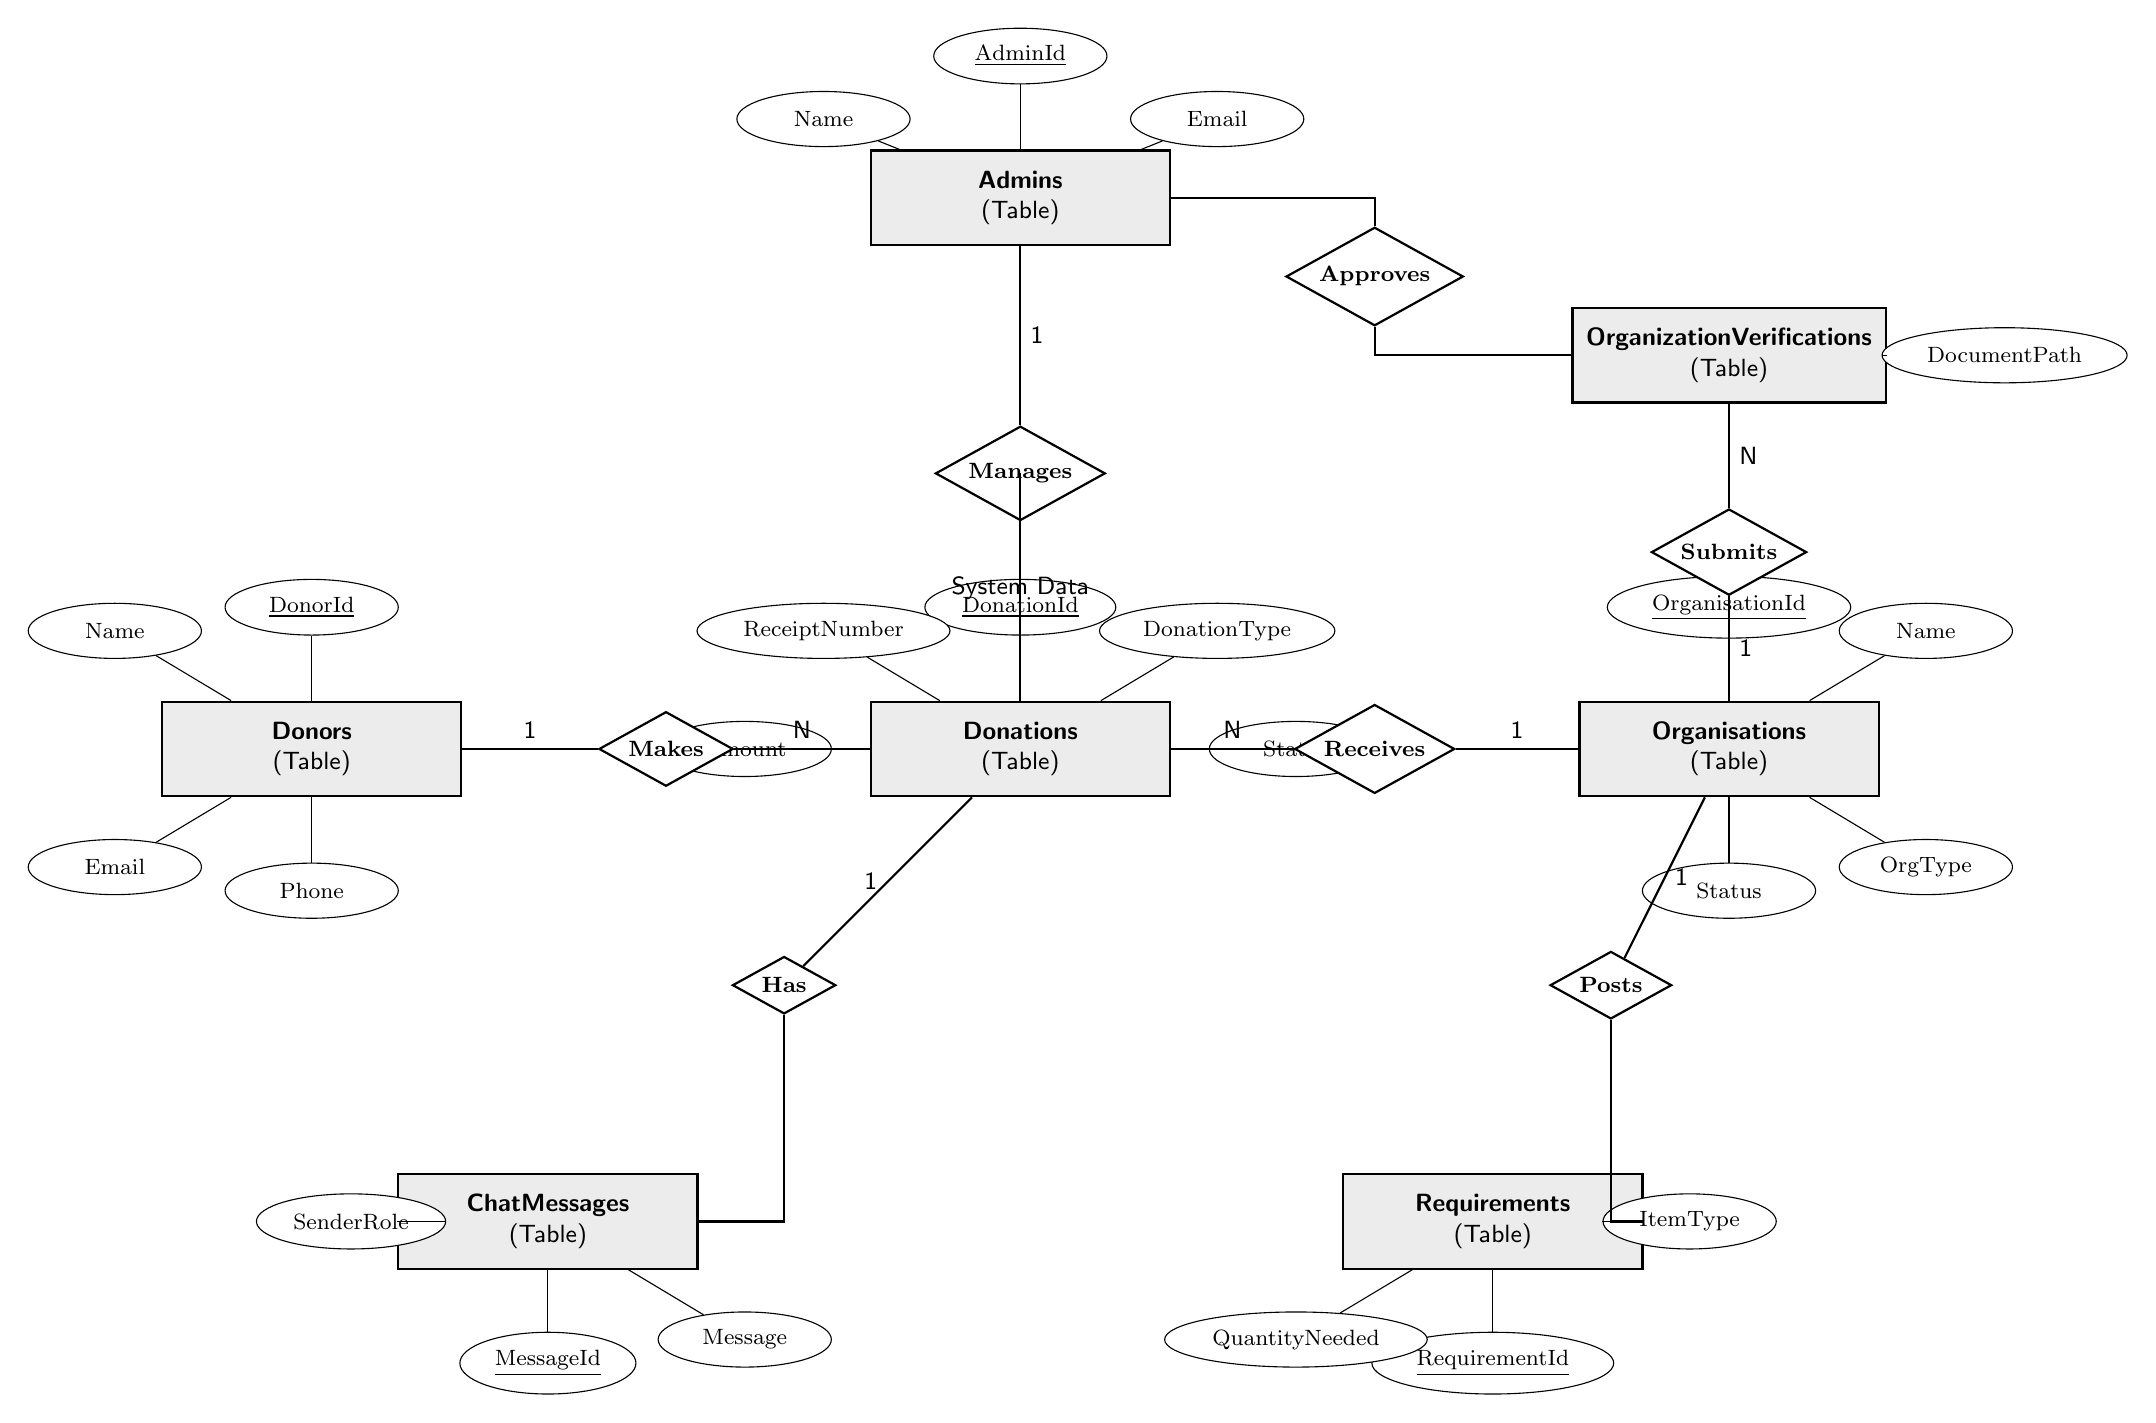
\begin{tikzpicture}[
    font=\sffamily\small,
    entity/.style={
        rectangle, draw=black, thick, 
        fill=gray!15, 
        minimum width=3.8cm, minimum height=1.2cm, align=center,
        inner sep=5pt
    },
    attribute/.style={
        ellipse, draw=black, thin, 
        fill=white, 
        minimum width=2.2cm, minimum height=0.7cm, align=center, font=\footnotesize
    },
    relationship/.style={
        diamond, draw=black, thick, 
        fill=white, 
        aspect=1.8, align=center, inner sep=2pt, font=\footnotesize\bfseries
    },
    line/.style={draw=black, thick}
]

% -------------------------
% 1. Core Transactional Center: DONATIONS
% -------------------------
\node[entity] (Donations) at (0, 0) {\textbf{Donations}\\(Table)};
\node[attribute] (Don1) at (0, 1.8) {\underline{DonationId}};
\node[attribute] (Don2) at (-2.5, 1.5) {ReceiptNumber};
\node[attribute] (Don3) at (2.5, 1.5) {DonationType};
\node[attribute] (Don4) at (-3.5, 0) {Amount};
\node[attribute] (Don5) at (3.5, 0) {Status};
\draw (Donations) -- (Don1); \draw (Donations) -- (Don2); \draw (Donations) -- (Don3); \draw (Donations) -- (Don4); \draw (Donations) -- (Don5);

% -------------------------
% 2. Main Actors: DONORS & ORGANISATIONS
% -------------------------
% DONORS (Left)
\node[entity] (Donors) at (-9, 0) {\textbf{Donors}\\(Table)};
\node[attribute] (Dor1) at (-9, 1.8) {\underline{DonorId}};
\node[attribute] (Dor2) at (-11.5, 1.5) {Name};
\node[attribute] (Dor3) at (-11.5, -1.5) {Email};
\node[attribute] (Dor4) at (-9, -1.8) {Phone};
\draw (Donors) -- (Dor1); \draw (Donors) -- (Dor2); \draw (Donors) -- (Dor3); \draw (Donors) -- (Dor4);

% ORGANISATIONS (Right)
\node[entity] (Organisations) at (9, 0) {\textbf{Organisations}\\(Table)};
\node[attribute] (Org1) at (9, 1.8) {\underline{OrganisationId}};
\node[attribute] (Org2) at (11.5, 1.5) {Name};
\node[attribute] (Org3) at (11.5, -1.5) {OrgType};
\node[attribute] (Org4) at (9, -1.8) {Status};
\draw (Organisations) -- (Org1); \draw (Organisations) -- (Org2); \draw (Organisations) -- (Org3); \draw (Organisations) -- (Org4);

% -------------------------
% 3. Management: ADMINS
% -------------------------
\node[entity] (Admins) at (0, 7) {\textbf{Admins}\\(Table)};
\node[attribute] (Adm1) at (0, 8.8) {\underline{AdminId}};
\node[attribute] (Adm2) at (-2.5, 8) {Name};
\node[attribute] (Adm3) at (2.5, 8) {Email};
\draw (Admins) -- (Adm1); \draw (Admins) -- (Adm2); \draw (Admins) -- (Adm3);

% -------------------------
% 4. Auxiliary: CHATMESSAGES & REQUIREMENTS
% -------------------------
% CHATMESSAGES (Bottom Left)
\node[entity] (ChatMessages) at (-6, -6) {\textbf{ChatMessages}\\(Table)};
\node[attribute] (Chat1) at (-6, -7.8) {\underline{MessageId}};
\node[attribute] (Chat2) at (-8.5, -6) {SenderRole};
\node[attribute] (Chat3) at (-3.5, -7.5) {Message};
\draw (ChatMessages) -- (Chat1); \draw (ChatMessages) -- (Chat2); \draw (ChatMessages) -- (Chat3);

% REQUIREMENTS (Bottom Right)
\node[entity] (Requirements) at (6, -6) {\textbf{Requirements}\\(Table)};
\node[attribute] (Req1) at (6, -7.8) {\underline{RequirementId}};
\node[attribute] (Req2) at (8.5, -6) {ItemType};
\node[attribute] (Req3) at (3.5, -7.5) {QuantityNeeded};
\draw (Requirements) -- (Req1); \draw (Requirements) -- (Req2); \draw (Requirements) -- (Req3);

% -------------------------
% 5. Verification: ORGANIZATIONVERIFICATIONS
% -------------------------
\node[entity] (Verifications) at (9, 5) {\textbf{OrganizationVerifications}\\(Table)};
\node[attribute] (Ver1) at (12.5, 5) {DocumentPath};
\draw (Verifications) -- (Ver1);

% -------------------------
% RELATIONSHIPS (The "Proper Flow")
% -------------------------

% Donor -> Donations
\node[relationship] (Rel1) at (-4.5, 0) {Makes};
\draw[line] (Donors) -- node[above] {1} (Rel1) -- node[above] {N} (Donations);

% Org -> Donations
\node[relationship] (Rel2) at (4.5, 0) {Receives};
\draw[line] (Organisations) -- node[above] {1} (Rel2) -- node[above] {N} (Donations);

% Donations -> Chat
\node[relationship] (Rel3) at (-3, -3) {Has};
\draw[line] (Donations) -- node[left] {1} (Rel3);
\draw[line] (Rel3) |- (ChatMessages);

% Org -> Requirements
\node[relationship] (Rel4) at (7.5, -3) {Posts};
\draw[line] (Organisations) -- node[right] {1} (Rel4);
\draw[line] (Rel4) |- (Requirements);

% Org -> Verifications
\node[relationship] (Rel5) at (9, 2.5) {Submits};
\draw[line] (Organisations) -- node[right] {1} (Rel5) -- node[right] {N} (Verifications);

% Admin -> Actors/Data
\node[relationship] (Rel6) at (0, 3.5) {Manages};
\draw[line] (Admins) -- node[right] {1} (Rel6);
\draw[line] (Rel6) -| node[above, pos=0.8] {System Data} (Donations);

\node[relationship] (Rel7) at (4.5, 6) {Approves};
\draw[line] (Admins) -- (4.5, 7) -- (Rel7) -- (4.5, 5) -- (Verifications);

\end{tikzpicture}
\end{document}
